  
% configuração da fonte, pode ser courier ou times

\documentclass[courier]{uninove-ppgi}

% local definitions (utilizado para controlar a posição do número da equação)

\newcommand{\numberequation}[1]{\addtocounter{equation}{#1}\tag{\theequation}}

    \begin{document}
    
        % parametros de capa e folha de rosto (é necessário configurar todos)
        
        \Universidade{UNIVERSIDADE NOVE DE JULHO - UNINOVE}
        \Programa{PROGRAMA DE PÓS GRADUAÇÃO EM INFORMÁTICA E GESTÃO DO CONHECIMENTO - PPGI} 	
        \Autor{GUILHERME BUENO \\ RAFAEL COTRIN \\ SAULO STOPA} 
        \Titulo{Relatório de comparação de desempenho do artigo: Application of The Fuzzy Inference System Method to Predict The Number of Weaving Fabric Production}
        \Tipoexame{Trabalho cientifico}
        \Titulacao{Mestre}
        \Orientador{Professor e Dr. Cleber}
        \Ano{2021}
    
    
    % gera a capa
    
        \capa
        
        
        % gera folha de rosto
        
        \folharosto
    
    		   
    % configurações do resumo em portugues
    
    \PalavrasChave{Sistema Fuzzy, Sistema Inteligente, Validar fuzzy, XXXXXXX, XXXXXXXXX.}
    
    \begin{resumo}
    
        Atendendo a solicitação de criação de trabalho junto a instituição Universidade Nove de Julho, para a matéria de Sistemas de Inferência Fuzzy (SIF),
        tendo como Professor responsável Prof. DR. Cleber. O proposto foi realizar uma pesquisa afim de identificar um artigo para que fosse simulado toda a estrutura de um SIF. 
        Sendo essa criação desenvolvida utilizando novo sistema, ou seja, sem utilização de softwares ou plugins prontos de mercado. Após essa elaboração, analisar
        as saídas do modelo de MANDANI com saídas de um sistema por Takagi-Sugeno, ou o inverso, identificando quais foram as melhores saídas olhando para o universo de 
        discurso e variáveis linguísticas escolhidas para o trabalho. O artigo escolhido buscou determinar aplicação da lógica fuzzy na resolução de problemas de produção usando o método de Tsukamoto e o Método de Sugeno \citeonline{tundo2018application}.
		O problema em específico foi determinar a produção de tecidos usando 3 variáveis como dados de entrada, sendo essas: estoque, demanda e estoque de custo de produção \citeonline{tundo2018application}.
		A abordagem a qual iremos utilizar é a de Takagi-Sugeno, não abordaremos a diferença entre essas duas técnicas descritas no artigo, onde iremos comparar apenas os resultados do método de Sugeno usado no artigo
		com o modelo de MANDANI que elaboramos. Comparar o desempenho de pelo menos três tipos diferentes de funções de pertinência, e para MANDANI realizar a comparação o desempenho de duas
		funções diferentes de defuzzificação. Por fim, escolher indicador de desempenho para comparar os dois modelos.
    
    \end{resumo}
    
    
    % configurações do resumo em inglês
    
    \KeyWords{Fuzzy System, Smart System, Validate fuzzy, XXXXXXX, XXXXXXXXX.}
    
    \begin{abstract}
    
        Responding to the request to create a work with the institution Nove de Julho University, for the subject of Fuzzy Inference Systems (SIF), having as responsible Prof. Dr. Cleber, the proposal was to carry out a research in order to identify an article so that the entire structure of a SIF could be simulated.
        This creation wasn't developed using software or market plug-ins, but development owned to analyze the output of the Mamdani models and Takagi-Sugeno, or the reverse, identifying which were the bests output, looking for at the universe of discourse and the linguistics variables. The chosen article sought to determine the application of fuzzy logic in solving production problems using the Tsukamoto method and the Sugeno method.
        The specific problem was to determine the fabric production using 3  input variables, namely: stock, demand and production cost of stock.
        The approach to compare used will be between the Takagi-Sugeno (described on the article) and our techniques developed using the Mamdani method, comparing the performance of at least three different types of membership functions.
        For the Mamdani method, we will to compare the performance of two different defuzzification functions, and finally, we will choose performance indicator to compare the two models.
    
    \end{abstract}
    
    % Sumário
    
    \tableofcontents 
    \thispagestyle{empty}
    		   
    % Lista de figuras
    
    \listoffigures
    \thispagestyle{empty}
    
    % Lista de algoritmos
    
    \listofalgorithms
    \thispagestyle{empty}
    
    % lista de abreviaturas (não colocar espaçamentos adicionais, pois eles contam dentro do environment)
    
    \begin{listaabreviaturas}%
    	SIF & Sistema de Inferência Fuzzy \\

    	\textit{poset} &  Acrônimo para a expressão em inglês \textit{partially ordered set}\\
    				   &  (em português: conjunto parcialmente ordenado) \\
    	\textit{pixel} &  Acrônimo para a expressão em inglês \textit{picture element}\\
    				   &  (em português: elemento da imagem)
    \end{listaabreviaturas}
    
    % lista de símbolos (não colocar espaçamentos adicionais, pois eles contam dentro do environment)
    % atualmente a lista não suporta multiplas páginas, ou seja ela quebra a lista inteira.
    
    \begin{listasimbolos}%
    	\simbolos{Conceitos básicos} {%		
    		$ \mathbb{Z} $ & Conjunto dos números inteiros \\						
    		$ \mathbb{N} $ & Conjunto dos números naturais \\		
    		$ \mathbb{R}^+ $ & Conjunto	dos números reais positivos \\	 		
    	}
    	\simbolos{Imagens} {%	
    		$ f $ & Váriavel que representa uma imagem \\			
    		$ \mathcal{D} $ & Conjunto que representa o domínio da imagem \\					
    		$ \mathbb{K} $ & Conjunto que representa o contradomínio da imagem \\		
    	}
    \end{listasimbolos}
    
    % Corpo do documento
    
    \chapter{Introdução}
    
        \begin{resumocapitulo}
            Este capítulo contempla Contextualização e Metodologia
        \end{resumocapitulo}
    
    \section{Contextualização}
    
        % Versão 1
		%Parágrafo
		A produção textil no mundo é algo indispensável existindo uma grande competição entre as empresas desse setor, onde acompanhar de perto a linha de produção para tomada de decisão faz toda a diferença.
		Quando se trata de vendas, pode-se relacionar uma cadeia de processos envolvidos onde se inicia no momento da solicitação do orçamento até a entrega do produto para o cliente final. Em todo esse processo
		existem técnologia e pessoas envolvidas, sendo que podem existir falhas capazes impactar diretamente o faturamento de uma empresa. No que diz respeito ao estoque, pode se definir como uma peça chave,
		pois, muitas vezes, para realizar uma venda precisa-se ter insumos já disponíveis para produção. Sendo assim, se uma empresa tem um estoque não controlado, sendo em excesso ou um baixo volume,
		podem trazer problemas financeiros \citeonline{tundo2018application}.
		O artigo escolhido tem como objetivo resolver problemas de produção de tecidos usando duas técnicas, Tsukamoto e Takagi-Sugeno. As variáveis de entrada para para criação dos univeros de discurso são: 
		estoque, demanda e estoque de custo de produção. A variável consequente ou de saída é a quantidade de produção de tecidos.

        
        % Parágrafo é destino a proposta
  
    
    \section{Metodologia}
    
	    Foi separada a montagem do trabalho em três etapas, sendo elas: (i) realizar uma pesquisa na literatura para identificar um artigo o qual fosse aderente ao trabalho; (ii) modelagem do código-fonte utilizando linguagem Python e a biblioteca numpy bem como a criação de métodos específicos para tratar cada um dos processos SIF; e (iii) realizar as inferências conforme solicitado no documento de requisitos para elaboração do seminário incluindo a comparação dos resultados obtidos nas simulações por meio de métrica de avaliação Erro quadrático. Confere a segunda etapa os seguintes processos: (a) Construção das funções de retas; (b) Fuzzificação; (c) Inferência; (e) Defuzzificação por Primeiro dos Máximos e Último dos Máximos.
		    
    
     \chapter{Etapa Um}
    
        \begin{resumocapitulo}
            Este capítulo resume de forma objetiva como foi elaborada a pesquisa na literatura afim de identificar o artigo usado neste relatório. 
        \end{resumocapitulo}
		
		\section{Revisão da Literatura}
		
    		Para a produção de modelo de sistema de inferência \textit{fuzzy} (SIF) implementado em código, foi realizada uma pesquisa na base de dados da \textit{CAPES} 
    		para identificar um artigo tal qual fosse facilmente reproduzível pelos dados fornecidos. E, como consequência da expressão de busca utilizada \textit{SYSTEM INFERENCE FUZZY} 
    		foi possível encontrar o artigo "\textit{Application of The Fuzzy Inference System Method to Predict The Number of Weaving Fabric Production}.
    		O artigo escolhido possui todas as características necessárias para validar o código construído: Fuzzificação; Inferência; Regras e Defuzzificação.
    		O mesmo também possui os dados de produção de tecidos utilizados no artigo, e são de fácil compreensão os universos de discurso assim como as variáveis linguísticas.
    
	
	\chapter{Etapa Dois}
    
        \begin{resumocapitulo}
            Este capítulo resume a etapa dois do processo a qual foram contruídos os métodos (a) Construção das funções de retas; (b) Fuzzificação; (c) Criação das regras; (d) Inferência; (e) Defuzzificação; (f) Função de agregação e (g) Cálculo do centroid.
        \end{resumocapitulo}
		
		\section{Construção das funções de retas}
		
		    % Descrição sobre as funções
		    A função de reta para extração dos coeficientes lineares $\theta_{0}$ e angulares $\theta_{1}$ das funções linguísticas utilizadas por \citeonline{tundo2018application} valeu-se, a princípio:
		    
		    \begin{proposicao}
		    
		        Dada uma equação de primeiro grau descrita por $y = \theta_{0} + \theta_{1}x$ onde $x$ e $y \in \mathbb{R}$ para os ponto $(x_{0}, y_{0})$ e $(x_{1}, y_{1})$, temos:
		        
		        \begin{equation}
		            \theta_{1} = \frac{y_{1} - y_{0}}{x_{1} - x_{0}}
		        \end{equation}
		        
		        \begin{equation}
		            \theta_{0} = y_{1} - \theta_{1}x_{1} 
		        \end{equation}
		        
		    \end{proposicao}
			 
			 Tal proposição sendo possível e equação implementável, foi desenvolvido o código da figura {Numero da figura}:
			 
			 % Inserir Figura
			 
		\section{Fuzzificação}
		
		     % Explicação da função fuzzify
			 Por meio da mesma equação descrita em \textbf{preposição 3.1} na seção \textbf{Construção das funções de retas}, é possível se chegar a uma lista de valores $y_{i}$, ou seja, uma lista de pertinências $\mu_{i}$ em situações em que dois pontos formam uma reta. Cada elemento $i$ das pertinências $\mu_{i}$, representa um termo linguístico. Assim, o comportamento da função de fuzzificação \textit{fuzzify}, para cada termo linguístico, equipara-se a:
			 
			 \begin{equation}
			     \mu_{i} = \begin{cases}
			        y_{0} \text{, se } x \leq x_{0} \\
			        \theta_{0} + \theta_1 \text{, se } x_{0} < x \leq x_{i} \\
			        y_{1} \text{, se } x > x_{1} \\
		        \end{cases}
			 \end{equation}
			 
			 % Explicação do código
			 O processo de fuzzificação constituirá, portanto, um processo que é definido em código conforme \textbf{figura \{Número da figura\}}. 
			 
			 
		     \begin{figure}[ht!]
    
        	    \begin{center}
        	
        		    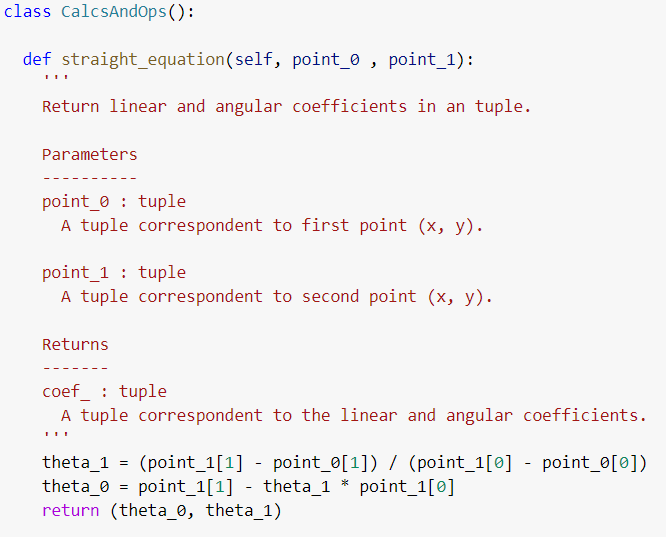
\includegraphics[scale=1]{straight equation}
        	
        	    \end{center}
        	
        	    \caption{Foto da função straight\_equation para extração dos coeficientes linares e angulares}
        	
        	\fonte{Elaborada pelo autor)}
        	
            \end{figure}

		\section{Inferência}
		
		     % Criação das regras
		     A criação das regras é efetuada pela função de inferência \textit{infer} que utiliza de recursividade para executar, em combinação de variáveis, sucessivas operações de minimização. Desta forma, em questão de combinação, opera-se em:
		     
		     \begin{equation}
                \begin{matrix}
                  \mu_{1,1} & \mu_{1,j} &  \mu_{1,m} \\
                  \vdots & \vdots &  \vdots \\
                  \mu_{i,1} & \mu_{i,j} & \mu_{i,m} \\
                  \vdots &  \vdots & \vdots \\
                  \mu_{n,1} & \mu_{n,j} & \mu_{n,m}
                \end{matrix}
		     \end{equation}
		     
		     Cada linha $i$ representada é uma variável linguística e $j$, representa cada termo linguístico correspondente a sua variável linguística. Deste modo, foi transcrita de acordo com a \textbf{figura \{numero da figura\}}.
		     
		     \begin{figure}[ht!]
    
        	    \begin{center}
        	
        		    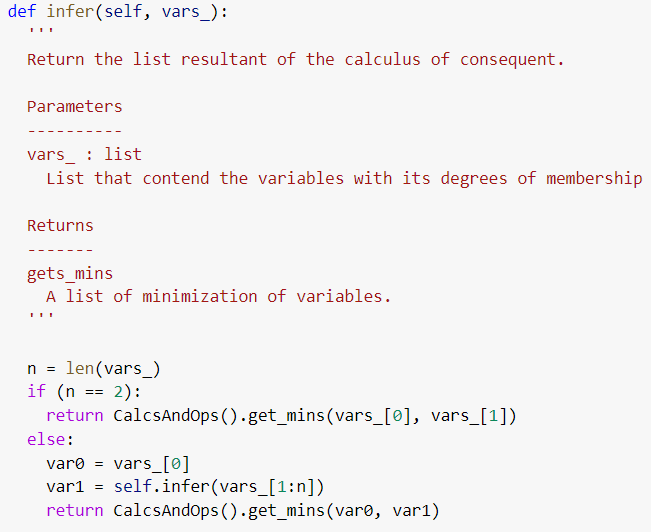
\includegraphics[scale=1]{infer}
        	
        	    \end{center}
        	
        	    \caption{Foto da função infer usada para inferir os graus de pertinência}
        	
        	\fonte{Elaborada pelo autor)}
        	
            \end{figure}
			
		\section{Defuzzificação}
		
			 % Explicação sobre a Defuzzificação pelo Primeiro dos Máximos
			 Dentre os métodos existentes de defuzzificação, foram se utilizados dois métodos conhecidos como o Primeiro dos Máximo, e o outro, Último dos máximo. O Primeiro dos Máximos, que tem, por conseguinte, o comportamento de retorna o menor valor da variável Crisp, ou da abcissa x,  segundo um valor de $\mu$. Não muito obstante desse entendimento, o método de defuzzificação por meio do Último dos Máximo utiliza abordagem inversa, tornando valore maiores de $x$ em relação a $\mu$.
			 
		     \begin{figure}[ht!]
    
        	    \begin{center}
        	
        		    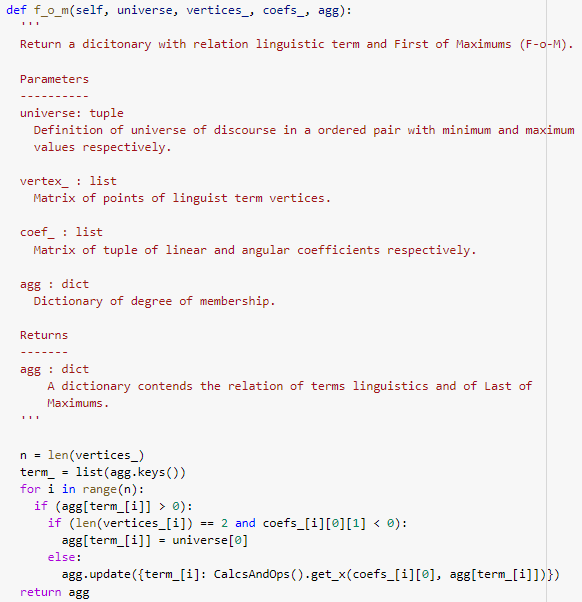
\includegraphics[scale=1.1]{f_o_m}
        	
        	    \end{center}
        	
        	    \caption{Foto da função f_o_m para extrair os valores dos Primeiros dos Máximos}
        	
        	\fonte{Elaborada pelo autor)}
        	
            \end{figure}
			 
			 
		     \begin{figure}[ht!]
    
        	    \begin{center}
        	
        		    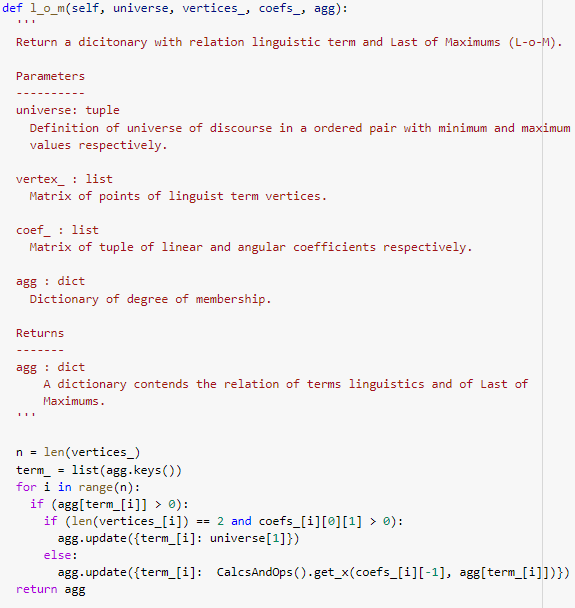
\includegraphics[scale=1.1]{l_o_m}
        	
        	    \end{center}
        	
        	    \caption{Foto da função l_o_m para extrair os valores dos Último dos Máximos}
        	
        	\fonte{Elaborada pelo autor)}
        	
            \end{figure}
			
			 
	\chapter{Etapa Três}
    
        \begin{resumocapitulo}
            Este capítulo iremos demostrar as análises das inferências que foram realizadas e também onde será demostrado os cálculos para comparação dos métodos. 
        \end{resumocapitulo}
		
		\section{Inferências}
		 
		Infelizmente, não foi possível efetuar uma reprodução completa e fidedigna do artigo, pois este faz uso de duas abordagens: Tsukamoto e Takage-Sugeno. Porém o motivo do insucesso em uma completa reprodução do artigo ocorreu pelo fato de que quando utilizado o método de inferência de Takage-Sugeno, havia a falta de algumas variáveis nas regras. Porém, tentou-se utilizar de valores que poderiam se aproximar dos resultados demonstrados no artigo. Com isso, há a proposta de da utilização de outros valores conforme tabela.
		
		\begin{table}[ht!]
		    \centering
		    \begin{tabular}{|c||c|c|c||c|c|c|} \hline
	            % Cabeçalho 1
		        \textbf{Tipo} &  \multicolumn{3}{c||}{\textbf{Entradas}} & \multicolumn{3}{c|}{\textbf{Saída}} \\
		        \hline \hline
		        % Cabeçalho 2
		        \textbf{Variáveis} & \textbf{Stoke} & \textbf{Demand} & \textbf{Cost} & \textbf{Takage} & \textbf{P-d-M} & \textbf{U-d-M} \\ \hline
		        % Linha 1
		        1 & 60 & 320 & 6000000 & 266.768 & 146.427 & 403.333 \\ \hline
		        % Linha 2
		        2 & 70 & 320 & 6000000 & 264.248 & 142.270 & 401.061 \\ \hline
		        % Linha 3
		        3 & 120 & 320 & 6000000 & 262.915 & 121.461 & 399.859 \\ \hline
		        % Linha 4
		        4 & 60 & 400 & 6000000 & 285.426 & 188.907 & 444.044 \\ \hline
		        % Linha 5
		        5 & 60 & 400 & 2450000 & 298.597 & 231.458 & 459.760 \\ \hline
		        % Linha 6
		        6 & 60 & 320 & 2450000 & 278.285 & 165.425 & 413.715 \\ \hline
		    \end{tabular}
		    \caption{Comparativa dos métodos de saída de Takage-Sugeno (Takage), Primeiro dos Máximos de Mamdani (P-d-M) e Último dos Máximos de Mamdani (U-d-M).}
		    \label{tab:my_label}
		\end{table}
		
	\chapter{Conclusões}
    
        \begin{resumocapitulo}
            Conclusões, Implicações e possíveis trabalhos futuros.
        \end{resumocapitulo}
		
		\section{Conclusões}
		
		 Descrição da conclusão....
		 
	     \begin{figure}[ht!]
    
    	    \begin{center}
    	
    		    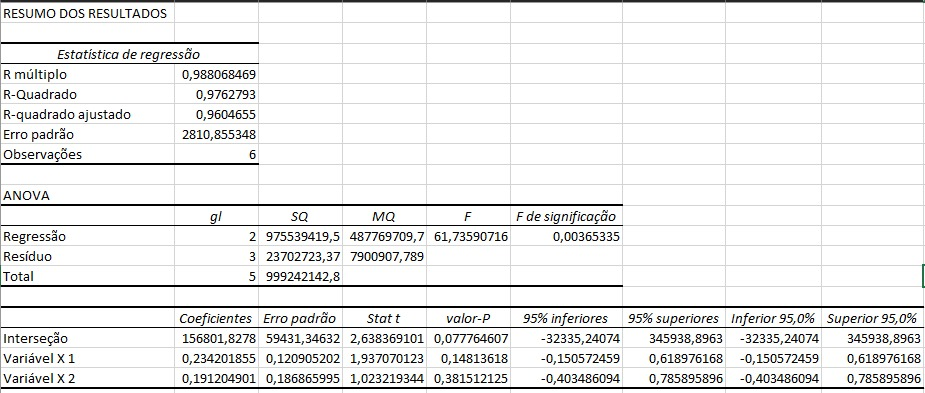
\includegraphics[scale=0.4]{WhatsApp Image 2021-06-24 at 05.51.07}
    	
    	    \end{center}
    	
    	    \caption{Análises comparativos feitas no Excel.}
    	
    	\fonte{Elaborada pelo autor)}
    	
    \end{figure}
     
    \subsubsection{Exemplo de subsubseção}
    
    Figuras também estão configuradas pela norma ABNT, a legenda é centralizada e a fonte da figura é recuada a esquerda:
    
    \begin{figure}[ht!]
    
    	\begin{center}
    	
    		
\includegraphics[scale=0.4]{leveling1}
    	
    	\end{center}
    	
    	\caption{Uma imagem.}
    	
    	\fonte{\citeonline{alves:article:2017} (Adaptado pelo autor)}
    	
    \end{figure}
    
    As citações podem ser feitas de duas formas: {\color{red}$\backslash$citeonline}\{chave da citação\} = \citeonline{seymor:book:1971} e {\color{red}$\backslash$cite}\{chave da citação\} = \cite{seymor:book:1971}. Note que, nas referências bibliográficas o título está em negrito, de acordo com a norma ABNT 6023, para este efeito é necessário incluir a entrada no arquivo bibtex (refs.bib).
    
    Exemplo simples de pseudocódigo utilizando o pacote {\color{red}algorithm2e} configurado para língua portuguesa:
    
    
    % Incluindo bibliografia
    
    \bibliography{refs}
    		   
    \end{document}
